\documentclass[aspectratio=169,10pt]{beamer}

\usetheme[
  color=red,
  font=lato,
  titlefont=avantgarde,
  footerlogo=hust,
  bar=thin,
  titlepage=cover,
  sectionpage=panel,
  numbering=fraction,
  progressbar=on,
  framebg=on
]{HUST}
\input{hust-setup}

\usepackage{amsmath,amssymb}
\usepackage{booktabs,graphicx,tabularx}
\usepackage[backend=biber,style=numeric,sorting=none,maxcitenames=2,mincitenames=1]{biblatex}
\addbibresource{references_revised.bib}
\graphicspath{{figures/}{../../HUST-Beamer-Theme/assets/}}

\usetikzlibrary{positioning,fit,backgrounds}
\tikzset{
  box/.style={rounded corners=1.5pt,align=center,inner sep=2pt,minimum height=.62cm,font=\scriptsize},
  frz/.style={box,draw=hustnavy,fill=hustnavy!8},
  mix/.style={box,draw=hustamber,fill=hustyellow!30,thick},
  trn/.style={box,draw=hustmain,fill=hustmain!18,thick},
  plain/.style={box,draw=none,fill=none},
  flow/.style={-{Latex[length=1.5mm]},thick,hustblack},
  gate/.style={-{Latex[length=1.5mm]},thick,hustmain},
  dict/.style={-{Latex[length=1.5mm]},thick,hustnavy},
  group/.style={rounded corners=3pt,draw=hustgray,dashed,inner sep=4pt},
  note/.style={font=\tiny,text=hustblack!80,align=center}
}
\newcommand{\legend}{%
  {\scriptsize\tikz\node[frz,minimum height=.22cm,minimum width=.35cm]{};~frozen\quad
  \tikz\node[mix,minimum height=.22cm,minimum width=.35cm]{};~input-conditioned\quad
  \tikz\node[trn,minimum height=.22cm,minimum width=.35cm]{};~trainable in FSFT}}

\title[WEMoE for NLP]{Merging BERT Experts with Weight-Ensembling MoE}
\subtitle{Few-shot router training across five GLUE tasks}
\author[Group 1]{Group 1\texorpdfstring{\\[2pt]}{ }{\small Nguyễn Bá Anh -- 20261218M\\ Nguyễn Thị Nhã Linh -- 20261262M}\texorpdfstring{\\[2pt]}{ }{\small\textcolor{blue!55!black}{Instructor: Nguyễn Kiêm Hiếu}}}
\institute{}
\date{}
\hypersetup{pdfauthor={Nguyễn Bá Anh; Nguyễn Thị Nhã Linh; Instructor: Nguyễn Kiêm Hiếu}}

\begin{document}

\begin{frame}[plain]
  \titlepage
\end{frame}

\begin{frame}{Motivation: one model, many task experts}
  \centering
  \begin{tikzpicture}[card/.style={box,minimum width=4.3cm,minimum height=1.45cm,font=\footnotesize}]
    \node[frz,card] (a) at (0,0) {\textbf{Five fine-tuned experts}\\ score \textbf{78.2}\quad 547.4M params\\ {\scriptsize strong, but five checkpoints}};
    \node[frz,card] (b) at (4.7,0) {\textbf{Task Arithmetic (static)}\\ score \textbf{57.4}\quad 109.5M params\\ {\scriptsize compact, but loses performance}};
    \node[mix,card] (c) at (9.4,0) {\textbf{WEMoE (input-conditioned)}\\ score \textbf{?}\quad storage \textbf{?}\\ {\scriptsize one merged model}};
  \end{tikzpicture}
  \raggedright
  \vfill
  \textbf{Question:} can input-conditioned MLP weights recover task performance with one merged model, at lower storage than five experts?
  \vfill
  \begin{block}{Scope}
    BERT/GLUE adaptation of WEMoE, not a reproduction of the paper's CLIP/image experiments.\cite{tang2024wemoe}
  \end{block}
\end{frame}

\begin{frame}{Theory: route in task-vector space}
  \centering
  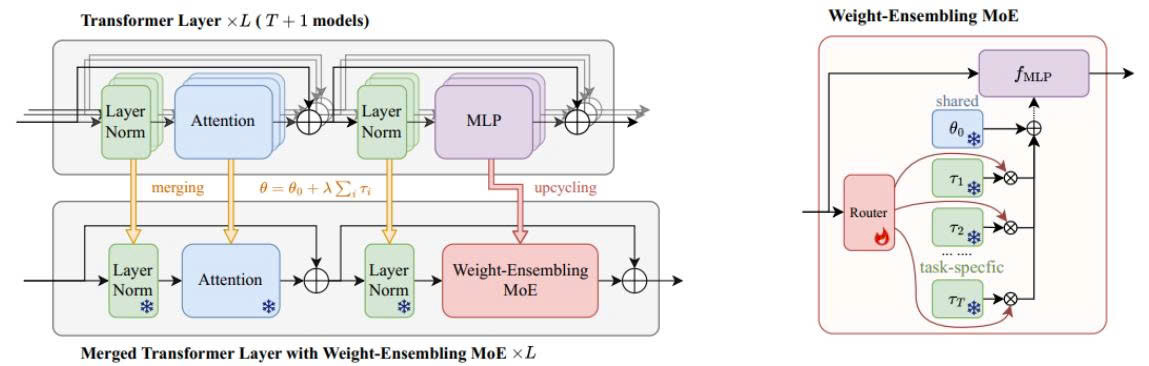
\includegraphics[width=.8\linewidth]{wemoe_paper.png}\\[-1pt]
  {\tiny Left: merge non-MLP blocks, upcycle MLPs. Right: WEMoE module. Figure from Tang et al.\ (CLIP-ViT, pre-norm layer).\cite{tang2024wemoe}}
  \vfill
  \footnotesize
  \begin{tabular}{ccc}
    Task vector & Non-MLP blocks (static) & MLP blocks (per input)\\[1pt]
    $\tau_e = W_e - W_0$ &
    $\theta = \theta_0 + \lambda\sum_{e}\tau_e$ &
    $W(x) = W_0 + \sum_{e=1}^{E} w_e(x)\,\tau_e$
  \end{tabular}
  \vfill
  \raggedright
  \begin{itemize}\footnotesize
    \item $W_0$: shared pretrained knowledge; $\tau_e$: task-specific change, the ``expert''.
    \item $w_e(x)$ are \textbf{unnormalised}: they may amplify or subtract task vectors.
  \end{itemize}
\end{frame}

\begin{frame}{Method: BERT MLPs become input-conditioned}
  \centering
  \begin{tikzpicture}[x=1cm,y=1cm]
    % data path
    \node[plain] (in) at (.45,0) {Tokens $x$\\ task $t$};
    \node[frz,minimum width=1.05cm] (emb) at (1.75,0) {Embed-\\dings};
    \node[frz,minimum width=1.35cm] (att) at (3.45,0) {Attention\\+ Add\&Norm};
    \node[mix,minimum width=1cm] (fc1) at (5.3,0) {fc1\\ $W^{\ell}_1(x)$};
    \node[frz,minimum width=.8cm] (act) at (6.45,0) {GELU};
    \node[mix,minimum width=1cm] (fc2) at (7.6,0) {fc2\\ $W^{\ell}_2(x)$};
    \node[frz,minimum width=.95cm] (nrm) at (8.95,0) {Add\\\&Norm};
    \node[frz,minimum width=.9cm] (pool) at (10.6,0) {Pooler\\ {[CLS]}};
    \node[frz,minimum width=.9cm] (head) at (11.95,0) {Head\\ $g_t$};
    \node[plain] (out) at (13.2,0) {Logits\\ $\to\hat y$};
    \foreach \a/\b in {in/emb,emb/att,att/fc1,fc1/act,act/fc2,fc2/nrm,nrm/pool,pool/head,head/out}
      \draw[flow] (\a) -- (\b);
    % offline sources
    \node[frz,minimum width=3.35cm] (ta) at (2.6,1.45) {Task Arithmetic, $\lambda=0.3$\\ $\theta=\theta_0+\lambda\sum_e\tau_e$};
    \node[frz,minimum width=3.3cm] (dict) at (6.45,1.45) {Dictionary per MLP layer\\ $W_0,\ \tau_{\text{MRPC}},\dots,\tau_{\text{QNLI}}$};
    \node[frz,minimum width=3.6cm] (src) at (11.1,1.45) {Pretrained $\theta_0$ + five experts $\theta_e$\\ (each expert also gives head $g_e$)};
    \draw[dict] (ta.south -| emb) -- (emb);
    \draw[dict] (ta.south -| att) -- (att);
    \draw[dict] (dict.south -| fc1) -- (fc1);
    \draw[dict] (dict.south -| fc2) -- (fc2);
    \draw[dict] (src.west) -- (dict.east);
    \draw[dict] (dict.west) -- (ta.east);
    \draw[dict] (src.south -| head) -- (head);
    % router
    \node[trn,minimum width=2.7cm] (rt) at (6.45,-1.28) {Router $r^{\ell}$ (one per layer)};
    \coordinate (tap) at ($(att.east)!.5!(fc1.west)$);
    \draw[gate] (tap) |- (rt.west);
    \node[note,anchor=east] at (tap |- rt.west) {token states $h_i$\ };
    \draw[gate] (rt.north -| fc1) -- (fc1.south);
    \draw[gate] (rt.north -| fc2) -- (fc2.south);
    \node[note,anchor=west] at (8.1,-1.28) {$w^{\ell}(x)\in\mathbb{R}^{5}$, shared by fc1 and fc2};
    % layer group
    \begin{scope}[on background layer]
      \node[group,fit=(att)(nrm)(rt)] (g) {};
    \end{scope}
    \node[note,anchor=north east] at (g.south east) {encoder layer $\ell$, $\times 12$};
  \end{tikzpicture}
  \vfill
  \legend
  \vfill
  \raggedright
  \begin{itemize}\footnotesize
    \item \textbf{Full} scope: fc1 + fc2 (\texttt{intermediate.dense}, \texttt{output.dense}). \textbf{Intermediate-only}: fc1; fc2 uses Task Arithmetic.
    \item All other weights use Task Arithmetic. Experts do \textbf{not} run at inference: one forward pass; the task id selects the head.
  \end{itemize}
\end{frame}

\begin{frame}{Components: frozen experts, trainable routers}
  \centering
  \begin{tikzpicture}[x=1cm,y=1cm]
    \node[anchor=west,font=\footnotesize\bfseries,text=hustnavy] at (-.1,.72) {Expert $e$: full fine-tune, then frozen};
    \node[plain] (i1) at (.45,0) {Tokens};
    \node[frz,minimum width=2cm] (b1) at (2.3,0) {BERT encoder $\theta_e$\\ 12 layers, hidden size $d$};
    \node[frz,minimum width=1cm] (p1) at (4.25,0) {Pooler};
    \node[frz,minimum width=1.5cm] (h1) at (5.85,0) {Head $g_e$\\ Dropout + Linear};
    \node[plain] (o1) at (7.5,0) {2 logits};
    \foreach \a/\b in {i1/b1,b1/p1,p1/h1,h1/o1} \draw[flow] (\a) -- (\b);
    \node[anchor=west,font=\scriptsize,text width=5.7cm] at (8.25,.1) {
      $f_e(x)=g_e\big(\mathrm{BERT}(x;\theta_e)\big)$\\[2pt]
      Output to WEMoE: task vectors $\tau_e$ and head $g_e$.\\
      Tasks: MRPC, RTE, CoLA, SST-2, QNLI.};
    \node[anchor=west,font=\footnotesize\bfseries,text=hustmain] at (-.1,-.95) {Router $r^{\ell}$: one per layer, 7.1M parameters in total};
    \node[plain] (i2) at (.45,-1.67) {$h_i\in\mathbb{R}^{d}$};
    \node[trn,minimum width=1.05cm] (f1) at (1.85,-1.67) {Linear\\ $d\to d$};
    \node[trn,minimum width=.65cm] (re) at (3.05,-1.67) {ReLU};
    \node[trn,minimum width=1.05cm] (f2) at (4.25,-1.67) {Linear\\ $d\to 5$};
    \node[frz,minimum width=1cm] (mm) at (5.75,-1.67) {Masked\\ mean};
    \node[plain] (o2) at (7.3,-1.67) {$w^{\ell}(x)\in\mathbb{R}^{5}$};
    \foreach \a/\b in {i2/f1,f1/re,re/f2,f2/mm,mm/o2} \draw[gate] (\a) -- (\b);
    \node[anchor=west,font=\scriptsize,text width=5.7cm] at (8.25,-1.75) {
      $r(h)=A_2\,\mathrm{ReLU}(A_1h+b_1)+b_2$\\[2pt]
      $w^{\ell}(x)=\dfrac{\sum_i m_i\,r^{\ell}(h_i)}{\sum_i m_i}$\quad ($m_i$: non-padding mask)};
  \end{tikzpicture}
  \vfill
  \raggedright
  \begin{itemize}\footnotesize
    \item \textbf{No softmax, no top-$k$:} $w^{\ell}(x)$ is a dense real-valued vector, not a probability distribution.
    \item \textbf{Initialisation:} $b_2=\lambda$, small $A_1,A_2$, so $w_e(x)\approx\lambda$ and the model starts near Task Arithmetic.
    \item \textbf{Per-sample merge:} the same $w^{\ell}(x)$ mixes weights and biases of the layer's upscaled modules.
  \end{itemize}
\end{frame}

\begin{frame}{Pipeline: what each stage optimises or computes}
  \centering
  \scriptsize
  \renewcommand{\arraystretch}{1.5}
  \begin{tabularx}{\linewidth}{>{\bfseries}p{2.25cm} p{1.15cm} X p{1.75cm}}
    \toprule
    Stage & Phase & Equation & Updates\\
    \midrule
    1.\ Fine-tune experts & Training &
    $\displaystyle\min_{\theta_e,\,g_e}\ \mathbb{E}_{(x,y)\sim D_e}\big[-\log p(y\mid x;\theta_e,g_e)\big],\quad p=\mathrm{softmax}\,f_e(x)$ &
    One expert\\
    2.\ Merge & Build &
    $\tau_e=\theta_e-\theta_0;\quad \theta_{\text{non-MLP}}=\theta_0+\lambda\sum_e\tau_e$ &
    None\\
    3.\ FSFT & Training &
    $\displaystyle\min_{\phi}\ \sum_{t=1}^{5}\frac{1}{|B_t|}\sum_{(x,y)\in B_t}-\log p_\phi(y\mid x,t)$ &
    Routers $\phi$ only\\
    4.\ Predict & Inference &
    $W^{\ell}(x)=W_0^{\ell}+\sum_e w_e^{\ell}(x)\,\tau_e^{\ell};\quad \hat y=\arg\max_c\,\mathrm{softmax}\big(g_t(\mathrm{BERT}_{W(x)}(x))\big)_c$ &
    None\\
    \bottomrule
  \end{tabularx}
  \vfill
  \raggedright
  \begin{itemize}\footnotesize
    \item $B_t$: batch of 16 from $k$ few-shot examples of task $t$. AdamW, lr $10^{-4}$, 10\% warmup, 500 steps.
    \item The paper trains routers by unlabelled entropy minimisation (TTA); this project uses labelled cross-entropy.\cite{tang2024wemoe}
  \end{itemize}
\end{frame}

\begin{frame}{Data boundary: reserve router examples, select on dev}
  \centering
  \small
  \begin{tabularx}{\linewidth}{>{\bfseries}p{3.2cm} p{4cm} X}
    \toprule
    Portion of each official GLUE train split & Size & Used for\\
    \midrule
    \texttt{expert\_train} & Remaining examples & Fine-tune the task experts\\
    \texttt{fewshot\_pool} & 256 per task & FSFT router training only\\
    \texttt{dev} & 10\%, at most 1,000 & Choose expert epoch, $\lambda$, and router step\\
    Official validation & Task-specific & Final metrics only\\
    \bottomrule
  \end{tabularx}
  \vfill
  \begin{block}{Leakage control}
    Experts never see the few-shot pool or dev; official validation is never used for selection.
  \end{block}
\end{frame}

\begin{frame}{Experiments: compare merging, routing, and expert limits}
  \centering
  \footnotesize
  \begin{tabular}{l l l}
    \toprule
    Model & Merge rule & Selection / training\\
    \midrule
    Majority class & Constant prediction & None\\
    Simple Averaging & $\theta_0+\tfrac15\sum_e\tau_e$ & None\\
    Task Arithmetic & $\theta_0+\lambda\sum_e\tau_e$ & $\lambda$ on dev (best 0.3)\\
    WEMoE init & $w_e(x)\approx\lambda$ & Router initialisation only\\
    WEMoE + FSFT & $W_0+\sum_e w_e(x)\tau_e$ & CE on $k$ per task; dev every 50 steps, up to 500\\
    Five experts & No merge & Best epoch on dev\\
    \bottomrule
  \end{tabular}
  \vfill
  \begin{block}{Task score ($\times 100$)}
    MRPC: mean of accuracy and F1; CoLA: Matthews correlation (MCC); RTE, SST-2, QNLI: accuracy.
  \end{block}
  {\scriptsize Task Arithmetic: Ilharco et al.\cite{ilharco2023task}}
\end{frame}

\begin{frame}{Main result: FSFT recovers much of the merging gap}
  \centering
  \begin{tabular}{l r}
    \toprule
    Model & Average task score\\
    \midrule
    Majority class & 45.8\\
    Simple Averaging ($\lambda=1/5$) & 53.3\\
    Task Arithmetic ($\lambda=0.3$) & 57.4\\
    WEMoE init (before FSFT) & 57.8 $\pm$ 0.6\\
    WEMoE + FSFT, full MLP ($k=256$) & \textbf{69.9 $\pm$ 0.1}\\
    Five single-task experts & 78.2\\
    \bottomrule
  \end{tabular}
  \vfill
  \raggedright
  \begin{itemize}\footnotesize
    \item Gain over majority $=\frac{\text{score}-\text{majority}}{\text{expert}-\text{majority}}$: Task Arithmetic \textbf{18\%}, WEMoE + FSFT \textbf{59\%}.
    \item Router initialisation alone does not help (57.8): the gain comes from FSFT.
    \item Mean $\pm$ std over router seeds 0, 1, 2.
  \end{itemize}
\end{frame}

\begin{frame}{Few-shot budget: $k=256$ is stable, small $k$ is not}
  \centering
  \begin{tabular}{r r r r}
    \toprule
    $k$ per task & Avg score & Gain over majority & CoLA MCC\\
    \midrule
    16 & 60.8 $\pm$ 2.7 & 25.5\% & 27.6 $\pm$ 14.1\\
    64 & 64.6 $\pm$ 3.7 & 46.7\% & 20.5 $\pm$ 17.8\\
    256 & \textbf{69.9 $\pm$ 0.1} & 59.1\% & 42.6 $\pm$ 0.9\\
    \bottomrule
  \end{tabular}
  \vfill
  \raggedright
  \begin{itemize}
    \item Full-MLP WEMoE; mean $\pm$ std over router seeds 0, 1, 2.
    \item Small $k$ overfits early (best dev step 50--250 of 500) and varies across seeds.
    \item $k=16\to64$: average +3.8, gain almost doubles; part of the $k=16$ average is MRPC/RTE at constant-guess level.
  \end{itemize}
\end{frame}

\begin{frame}{Per-task results: aggregate gains hide a task trade-off}
  \centering
  \scriptsize
  \begin{tabular}{l c c c c c}
    \toprule
    & MRPC acc/F1 & RTE acc & CoLA MCC & SST-2 acc & QNLI acc\\
    \midrule
    Majority & 68.4/81.2 & 52.7 & 0.0 & 50.9 & 50.5\\
    Full MLP, $k=256$ & 76.3 $\pm$ 4.5 / 83.9 $\pm$ 2.8 & 52.0 $\pm$ 4.4 & 42.6 $\pm$ 0.9 & 88.0 $\pm$ 0.5 & 86.7 $\pm$ 0.7\\
    Intermediate, $k=256$ & 66.5 $\pm$ 0.7 / 76.6 $\pm$ 1.0 & 59.0 $\pm$ 0.9 & 41.7 $\pm$ 0.9 & 86.7 $\pm$ 0.2 & 86.5 $\pm$ 0.2\\
    Five experts & 82.1/88.1 & 63.2 & 59.1 & 92.2 & 91.2\\
    \bottomrule
  \end{tabular}
  \vfill
  \begin{alertblock}{Do not read the mean as universal dominance}
    Full MLP is below the RTE majority (52.0 vs.\ 52.7). Intermediate-only improves RTE but is below the MRPC majority (66.5/76.6 vs.\ 68.4/81.2).
  \end{alertblock}
  \vspace{-2pt}
  {\scriptsize RTE ($n=277$) and MRPC ($n=408$): standard error about 3 and 2 points, so part of the gap may be noise.}
\end{frame}

\begin{frame}{Storage trade-off: intermediate-only is smaller, not uniformly better}
  \centering
  \begin{tabular}{l r r r l}
    \toprule
    Deployment & Stored params & vs.\ five models & Avg score & Task contrast\\
    \midrule
    Five experts & 547.4M & 100\% & 78.2 & Strongest average\\
    WEMoE, full MLP & 400.0M & 73.1\% & 69.9 $\pm$ 0.1 & MRPC 76.3; RTE 52.0\\
    WEMoE, intermediate & 258.4M & 47.2\% & 69.1 $\pm$ 0.1 & MRPC 66.5; RTE 59.0\\
    \bottomrule
  \end{tabular}
  \vfill
  \raggedright
  \begin{itemize}\footnotesize
    \item Intermediate-only: \textbf{35\% fewer parameters} than full MLP, similar average; best step is late (400--500 of 500).
    \item \textbf{Caveat:} each task keeps its own head, so the task is known at inference. Five experts are then more accurate and only 37\% larger than full MLP.
    \item The storage case rests on intermediate-only, or on settings with unknown task.
    \item FSFT on one Tesla T4: 14--16 min (full), 8.5 min (intermediate); training time, not inference latency.
  \end{itemize}
\end{frame}

\begin{frame}{Routing: shared structure, and why full-MLP fails on RTE}
  \centering
  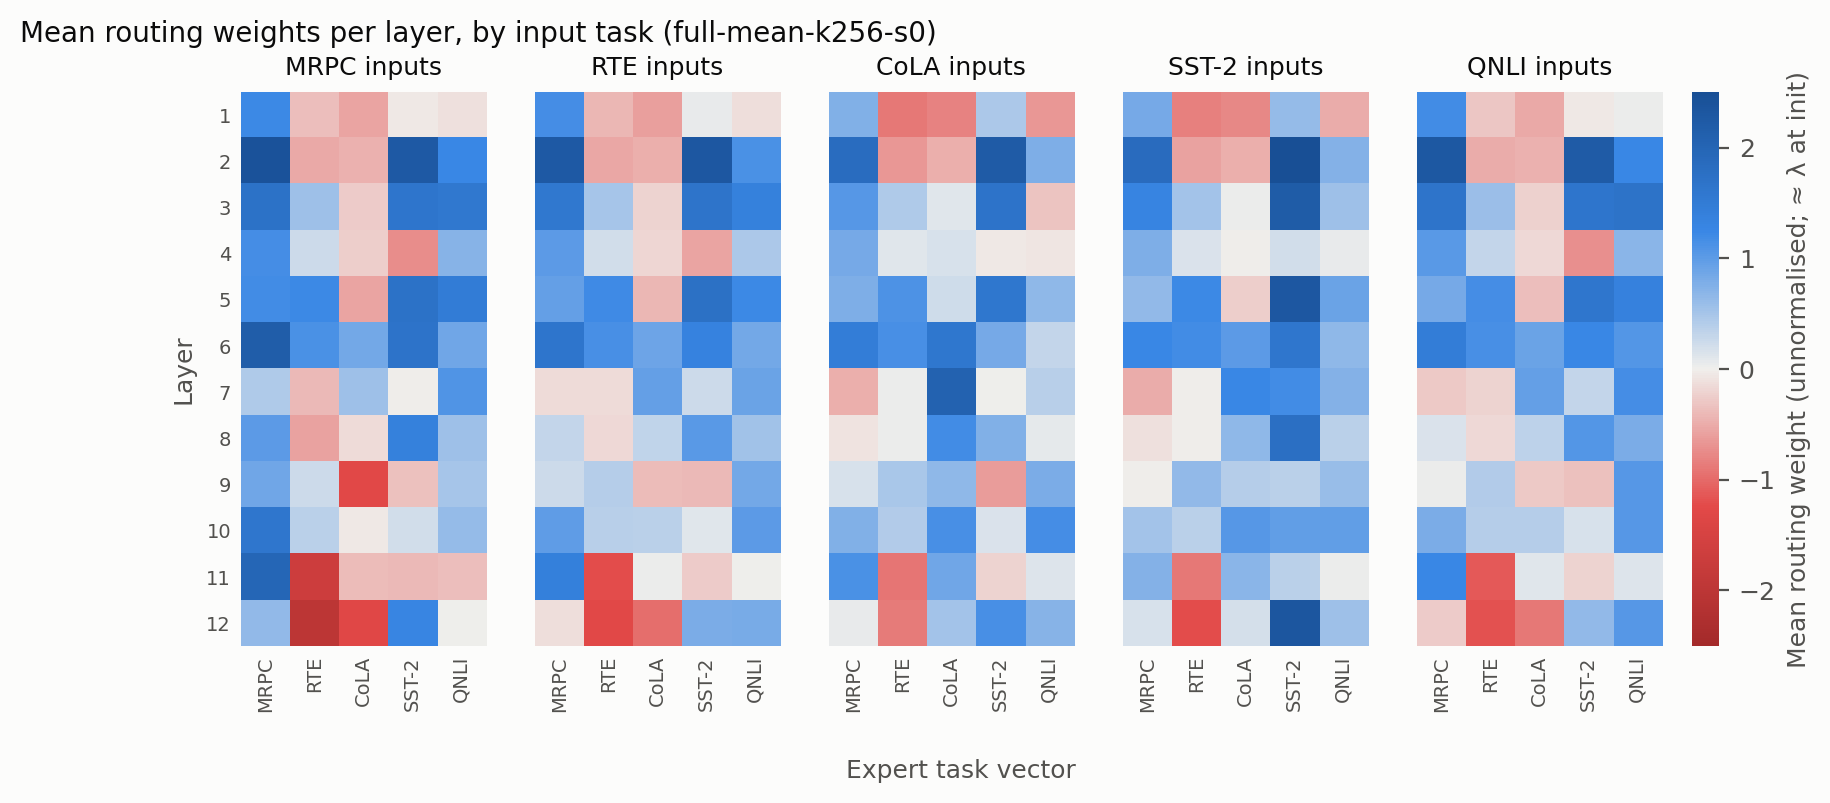
\includegraphics[width=0.96\linewidth,height=0.46\textheight,keepaspectratio]{routing.png}\par
  \vspace{-2pt}
  \raggedright
  \begin{itemize}\footnotesize
    \item \textbf{Shared pattern:} mean-matrix correlation 0.82; input task explains about 58\% of variance; weights span $-3.0$ to $4.4$.
    \item \textbf{RTE, full MLP:} own expert weight $\approx 0.01$ (MRPC: 1.37), and $-1.2$ in layers 11--12. Intermediate-only: 0.96, RTE 59.0.
  \end{itemize}
  {\scriptsize Full MLP, $k=256$, seed 0. Input-independent ablation pending: this plot does not show that input dependence causes the gains.}
\end{frame}

\begin{frame}{Limitations: encouraging aggregate, unresolved failures}
  \begin{itemize}
    \item \textbf{RTE failure:} full MLP 52.0, below the 52.7 majority; the RTE expert is also weak (63.2).
    \item \textbf{Small budgets vary:} at $k=16$, CoLA MCC std is 14.1 across router seeds.
    \item \textbf{Selection sees more labels:} up to 1,000 dev examples per task vs.\ $k=256$ for FSFT.
    \item \textbf{Limited seeds:} one seed for experts and data split.
  \end{itemize}
  \vfill
  \centering
  \small Paper: CLIP/image tasks, unlabelled test-time entropy minimisation. Here: 256 labelled examples per task. Comparison is qualitative.\cite{tang2024wemoe}
\end{frame}

\begin{frame}{Conclusion: WEMoE helps, but the task-level trade-offs matter}
  \begin{block}{Answer}
    In this first full BERT/GLUE run, few-shot router training raises the average to 69.9 (Task Arithmetic: 57.4; experts: 78.2).
  \end{block}
  \begin{itemize}
    \item Full MLP and intermediate-only: similar averages, different storage and per-task outcomes.
    \item RTE stays below majority for full MLP; an aggregate does not imply per-task dominance.
    \item Next: more seeds, stricter few-shot selection, routing ablation, inference latency.
  \end{itemize}
\end{frame}

% ---------------------------------------------------------------- Backup
\begin{frame}{Backup: Transformer architecture}
  \begin{columns}[T,onlytextwidth]
    \begin{column}{.33\textwidth}
      \centering
      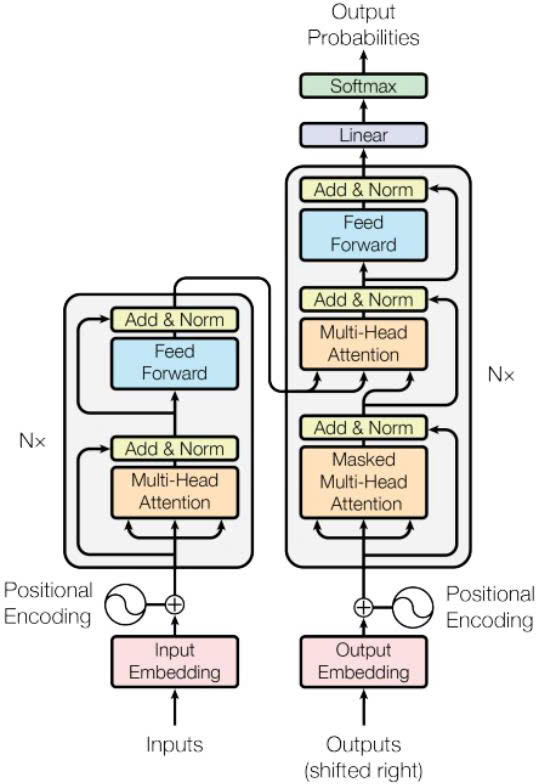
\includegraphics[height=5.5cm,keepaspectratio]{transformer_paper.png}\\[-1pt]
      {\tiny Figure: Vaswani et al.\cite{vaswani2017attention}}
    \end{column}
    \begin{column}{.65\textwidth}
      \footnotesize
      \textbf{Encoder:} self-attention + FFN. \textbf{Decoder:} adds masked self-attention and cross-attention.
      \vspace{3pt}

      \textbf{Self-attention}
      \[\mathrm{Attention}(Q,K,V)=\mathrm{softmax}\Big(\frac{QK^{\top}}{\sqrt{d_k}}\Big)V\]
      \textbf{Multi-head attention}
      \[\mathrm{MultiHead}(Q,K,V)=\mathrm{Concat}(\mathrm{head}_1,\dots,\mathrm{head}_h)W^{O}\]
      \textbf{Positional encoding:} sinusoidal vectors added to the embeddings, because attention does not encode order.
      \vspace{3pt}

      \textbf{FFN and residual}
      \[\mathrm{FFN}(x)=\max(0,xW_1+b_1)W_2+b_2,\quad y=\mathrm{LayerNorm}\big(x+\mathrm{Sublayer}(x)\big)\]
    \end{column}
  \end{columns}
\end{frame}

\begin{frame}{Backup: BERT architecture}
  \centering
  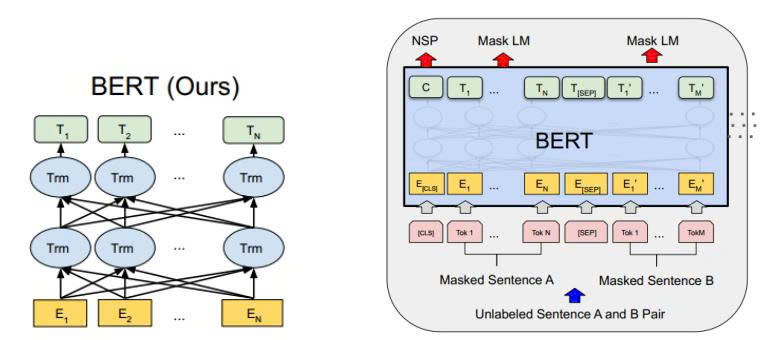
\includegraphics[width=.56\linewidth]{bert_paper.png}\\[-1pt]
  {\tiny Figure: Devlin et al.\ (encoder stack; MLM and NSP pre-training).\cite{devlin2019bert}}
  \vfill
  \raggedright
  \footnotesize
  \begin{columns}[T,onlytextwidth]
    \begin{column}{.5\textwidth}
      \begin{itemize}
        \item Encoder-only, bidirectional context.
        \item Input: \texttt{[CLS]} A \texttt{[SEP]} B \texttt{[SEP]}.
        \item $E=E_{\text{token}}+E_{\text{segment}}+E_{\text{position}}$ (learned positions).
      \end{itemize}
    \end{column}
    \begin{column}{.48\textwidth}
      \begin{itemize}
        \item Pre-training: MLM (predict masked tokens), NSP.
        \item \texttt{bert-base-uncased}: 12 layers, GELU.
        \item This project starts from the encoder and pooler only, with new 2-class heads.
      \end{itemize}
    \end{column}
  \end{columns}
\end{frame}

\begin{frame}{Backup: BERT fine-tuning for GLUE tasks}
  \centering
  \scriptsize
  \begin{tabular}{l l l l c}
    \toprule
    Task & Input & Label & Task score & Expert score\\
    \midrule
    MRPC & Sentence pair & not equivalent / equivalent & mean(acc, F1) & 85.1\\
    RTE & Sentence pair & entailment / not entailment & Accuracy & 63.2\\
    CoLA & One sentence & unacceptable / acceptable & MCC & 59.1\\
    SST-2 & One sentence & negative / positive & Accuracy & 92.2\\
    QNLI & Question + sentence & entailment / not entailment & Accuracy & 91.2\\
    \bottomrule
  \end{tabular}
  \vfill
  \begin{tabular}{l l l}
    \toprule
    & Pretrained BERT, $\theta_0$ & Fine-tuned expert, $\theta_e$\\
    \midrule
    Objective & Self-supervised MLM + NSP & Cross-entropy on one GLUE task\\
    Head & None kept & Dropout + Linear ($d\to2$) on pooled \texttt{[CLS]}\\
    Updated & -- & All BERT layers and the head\\
    Role in WEMoE & Shared base $W_0$, $\theta_0$ & Task vector $\tau_e=\theta_e-\theta_0$, head $g_e$\\
    \bottomrule
  \end{tabular}
  \vfill
  \raggedright
  \begin{itemize}\footnotesize
    \item One recipe for all tasks: AdamW, lr $2\times10^{-5}$, batch 32, 3 epochs, 10\% warmup, weight decay 0.01, length 128.
    \item All five tasks are binary classification, so no regression head is used.
  \end{itemize}
\end{frame}

\begin{frame}{Backup: weight ensembling vs.\ logit ensembling}
  \centering
  \begin{tikzpicture}[x=1cm,y=1cm]
    \node[anchor=west,font=\scriptsize\bfseries] at (0,1.0) {Logit ensembling (concept only)};
    \node[plain] (lx) at (.3,0) {$x$};
    \node[frz,minimum width=1.5cm,minimum height=.42cm] (e1) at (1.9,.48) {Model $\theta_1$};
    \node[plain,minimum height=.3cm] at (1.9,.04) {$\vdots$};
    \node[frz,minimum width=1.5cm,minimum height=.42cm] (e5) at (1.9,-.48) {Model $\theta_E$};
    \node[frz,minimum width=1.25cm] (s) at (4.2,0) {$\sum_e G_e(x)\,f_e(x)$};
    \node[plain] (ly) at (5.9,0) {$\hat y$};
    \draw[flow] (lx) -- (e1.west); \draw[flow] (lx) -- (e5.west);
    \draw[flow] (e1.east) -- (s); \draw[flow] (e5.east) -- (s); \draw[flow] (s) -- (ly);
    \node[anchor=west,font=\scriptsize\bfseries] at (7.2,1.0) {Weight ensembling (WEMoE)};
    \node[plain] (wx) at (7.5,0) {$x$};
    \node[trn,minimum width=1cm,minimum height=.42cm] (r) at (9,.48) {Router};
    \node[frz,minimum width=1cm,minimum height=.42cm] (d) at (9,-.48) {$W_0,\{\tau_e\}$};
    \node[mix,minimum width=2.1cm] (m) at (11.5,0) {One model\\ $W(x)=W_0+\sum_e w_e\tau_e$};
    \node[plain] (wy) at (13.6,0) {$\hat y$};
    \draw[flow] (wx) -- (r.west); \draw[gate] (r.east) -- (m.west); \draw[dict] (d.east) -- (m.west); \draw[flow] (m) -- (wy);
  \end{tikzpicture}
  \vfill
  \scriptsize
  \begin{tabularx}{\linewidth}{>{\bfseries}p{2.1cm} X X}
    \toprule
    & Logit ensembling & Weight ensembling\\
    \midrule
    Mixes & Model outputs & Parameters, inside each upscaled MLP\\
    Forward passes & One per expert & One, with per-sample weights\\
    Stored & Full models & Shared model + MLP task vectors (283M of 400M)\\
    Limitation & Cost grows with $E$; needs a shared output space & Storage for $\tau_e$; per-sample merge cost\\
    \bottomrule
  \end{tabularx}
  \vfill
  \raggedright
  \footnotesize
  For one linear layer, $W(x)h=W_0h+\sum_e w_e(\tau_e h)$. GELU and 12 stacked layers make the full model differ from a logit ensemble.
\end{frame}

\begin{frame}{Backup: router and Mixture of Experts}
  \centering
  \[
    \underbrace{\mathrm{MoE}(x)=\sum_{i=1}^{n}G_i(x)\,E_i(x)}_{\text{classic MoE: mixes expert outputs}}
    \qquad\longrightarrow\qquad
    \underbrace{h_{\text{out}}=f_{\text{MLP}}\big(h;\ W_0+D_{\tau}w(x)\big)}_{\text{WEMoE: mixes expert weights}}
  \]
  \vfill
  \footnotesize
  \begin{tabularx}{\linewidth}{>{\bfseries}p{2.5cm} X X}
    \toprule
    & Classic MoE & This project\\
    \midrule
    Experts & Trainable sub-networks & Frozen task vectors $\tau_e$ ($D_{\tau}$: dictionary)\\
    Gate output & Weight distribution; may keep top-$k$ & Unnormalised $w\in\mathbb{R}^5$; no softmax\\
    Routing & Often sparse: few experts active & \textbf{Dense}: all 5 task vectors in every layer\\
    Gate placement & Per MoE layer & One router per BERT layer; fc1, fc2 share $w$\\
    Training & Jointly with experts & Routers only, after experts are frozen\\
    \bottomrule
  \end{tabularx}
  \vfill
  \raggedright
  Negative weights are allowed: routing here is not a convex mixture of experts. Classic MoE as in Shazeer et al.\cite{shazeer2017moe}
\end{frame}

\begin{frame}{Backup: task metrics and aggregation}
  \begin{itemize}
    \item \textbf{MRPC:} mean of accuracy and F1. \textbf{CoLA:} MCC. \textbf{RTE, SST-2, QNLI:} accuracy.
    \item \textbf{Average score:} unweighted mean of five task scores, $\times 100$.
    \item \textbf{Uncertainty:} WEMoE mean $\pm$ std over router seeds 0, 1, 2; experts and data split fixed.
  \end{itemize}
\end{frame}

\begin{frame}{Backup: router training details}
  \begin{itemize}
    \item 256 labelled examples per task are reserved for FSFT; experts never see them.
    \item Router: two linear layers with ReLU, applied per token; outputs are averaged over non-padding tokens.
    \item AdamW, lr $10^{-4}$, batch 16 per task, up to 500 steps; 7.1M trainable parameters.
    \item Best step: dev every 50 steps, up to 1,000 examples per task.
    \item First full run: not a general guarantee or a complete reproduction of WEMoE.
  \end{itemize}
\end{frame}

\begin{frame}{Backup: WEMoE paper and this project}
  \centering
  \small
  \begin{tabularx}{\linewidth}{>{\bfseries}p{2.6cm} X X}
    \toprule
    & Tang et al. & This project\\
    \midrule
    Backbone, tasks & CLIP-ViT, 8 image tasks & BERT-base, 5 GLUE tasks\\
    Upscaled modules & Transformer MLPs & Full MLP; intermediate-only as ablation\\
    Routing input & Mean over tokens & Mean over non-padding tokens\\
    Router training & Entropy on unlabelled test data & Cross-entropy on $k$ labelled examples\\
    Router output & Unnormalised & Unnormalised, bias init $\lambda$\\
    Other parameters & Task Arithmetic, $\lambda=0.3$ & Task Arithmetic, $\lambda$ chosen on dev\\
    \bottomrule
  \end{tabularx}
  \vfill
  \raggedright
  The paper has no GLUE results, so the comparison is qualitative.\cite{tang2024wemoe}
\end{frame}

\begin{hustreferencesframe}[title={References},subtitle={}]
\end{hustreferencesframe}

\end{document}
